%%%%%%%%%%%%%%%%%%%%%%%%%%%%%%%%%%%%%%%%%%%%%%%%%%%%%%%%%%%%%%%%%%%
%                                                                 %
%  GEANT manual in LaTeX form                                     %
%                                                                 %
%  Michel Goossens (for translation into LaTeX)                   %
%  Version 1.00                                                   %
%  Last Mod. Jan 24 1991  1300   MG + IB                          %
%                                                                 %
%%%%%%%%%%%%%%%%%%%%%%%%%%%%%%%%%%%%%%%%%%%%%%%%%%%%%%%%%%%%%%%%%%%
\Origin{P.Zanarini}     
\Documentation{P.Zanarini, S.Giani, F.Carminati}      
\Submitted{01.11.83}       \Revised{13.12.93}
\Version{Geant 3.16}\Routid{DRAW220}
\Makehead{Drawing volume specifications}
The geometrical parameters of the volumes can be displayed via the 
\Rind{GDSPEC} routine (corresponding to the {\tt DSPEC} interactive 
command). This facility provides a detailed picture of a particular 
piece of the detector. 
The set of geometrical specifications 
of all the descendants of a given node on the tree, can be obtained
each on a separate picture with the routine \Rind{GDFSPC} ({\tt DFSPC} 
interactive command).

\Shubr{GDSPEC}{(CHNAME)}
\begin{DLtt}{MMMMMMMM}
\item[CHNAME] ({\tt CHARACTER*4}) volume name;
\end{DLtt}
Draws a picture showing all specifications for a given volume.
An example of use of \Rind{GDSPEC} can be found in Fig.~\ref{fg:draw220-1}.

\begin{figure}[hbt]
     \centering
     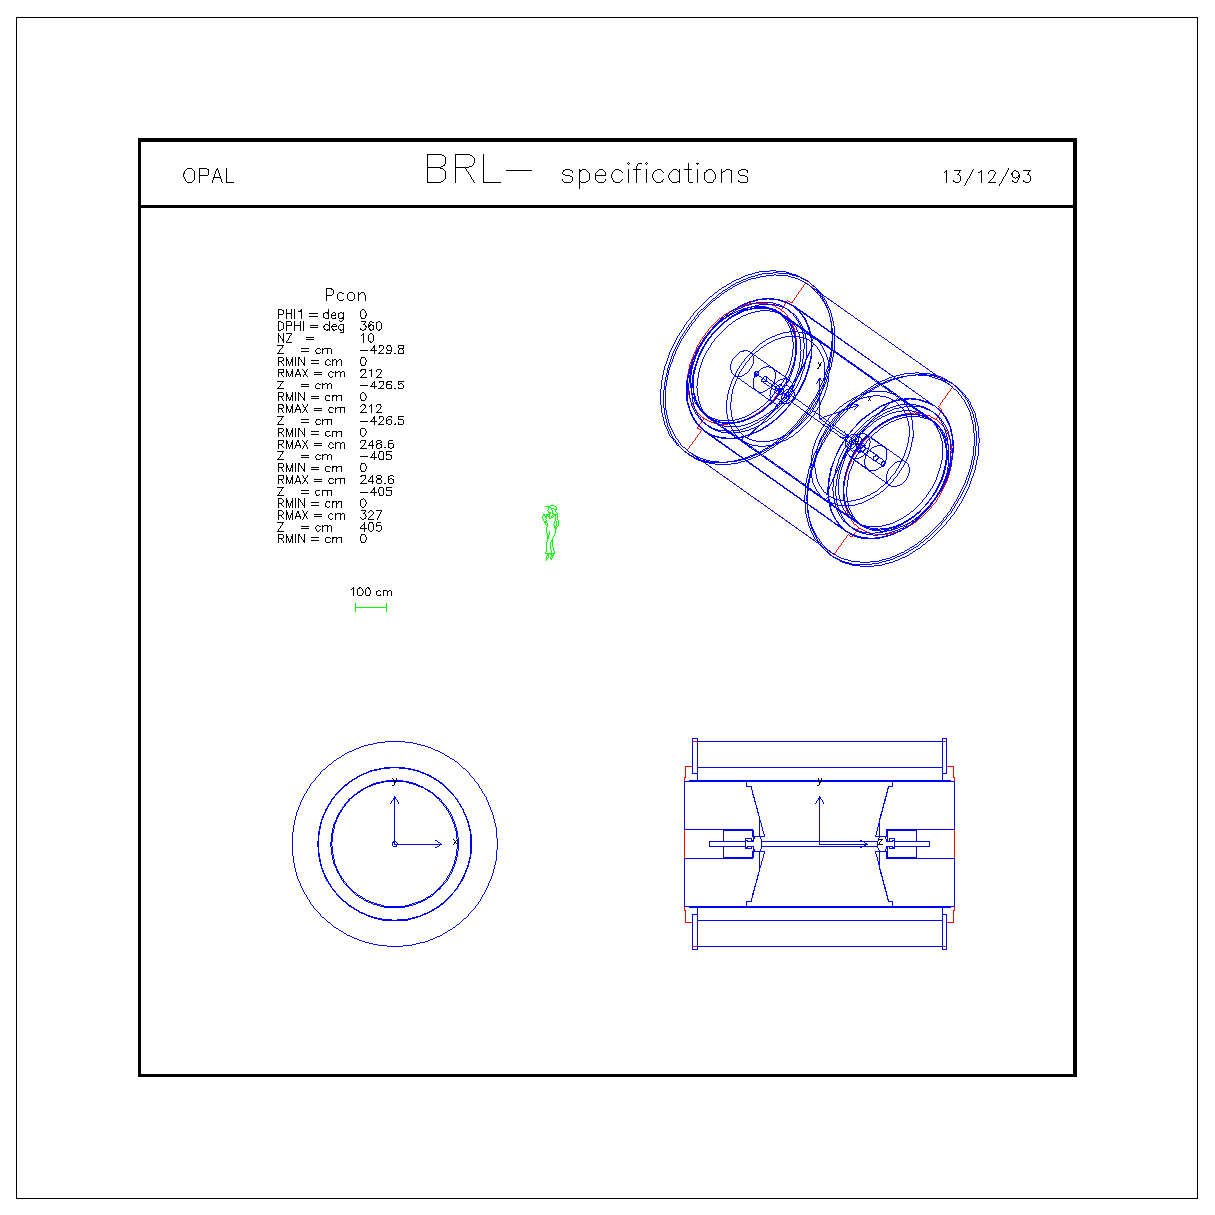
\epsfig{file=eps/draw220-1.eps,width=14cm}
     \caption{Example of use of {\tt GDSPEC}}
     \label{fg:draw220-1}
\end{figure}

The following information on the volume are
presented in a single frame:
\begin{itemize}
\item the volume daughters (one level down in the geometrical tree);
\item a space view of the volume (with $\theta$=45 and $\phi$=135);
\item a front view cut; 
\item a side view cut; 
\item the axes of the local coordinate system;
\item a human figure;
\item the scale;
\item the shape type;
\item all the numerical parameters that define the volume.
\end{itemize}
In drawing the volumes \Rind{GDSPEC} turns on the sets visibility 
({\tt 'SEEN'}) attribute for the volume {\tt CHNAME}
itself and its direct descendents. The setting of drawing options
({\tt HIDE}, {\tt CVOL}, {\tt FILL} $\ldots$) will be respected, allowing to 
customise the drawing. An example is shown in Fig.~\ref{fg:draw220-2}.
 
\begin{figure}[hbt]
     \centering
     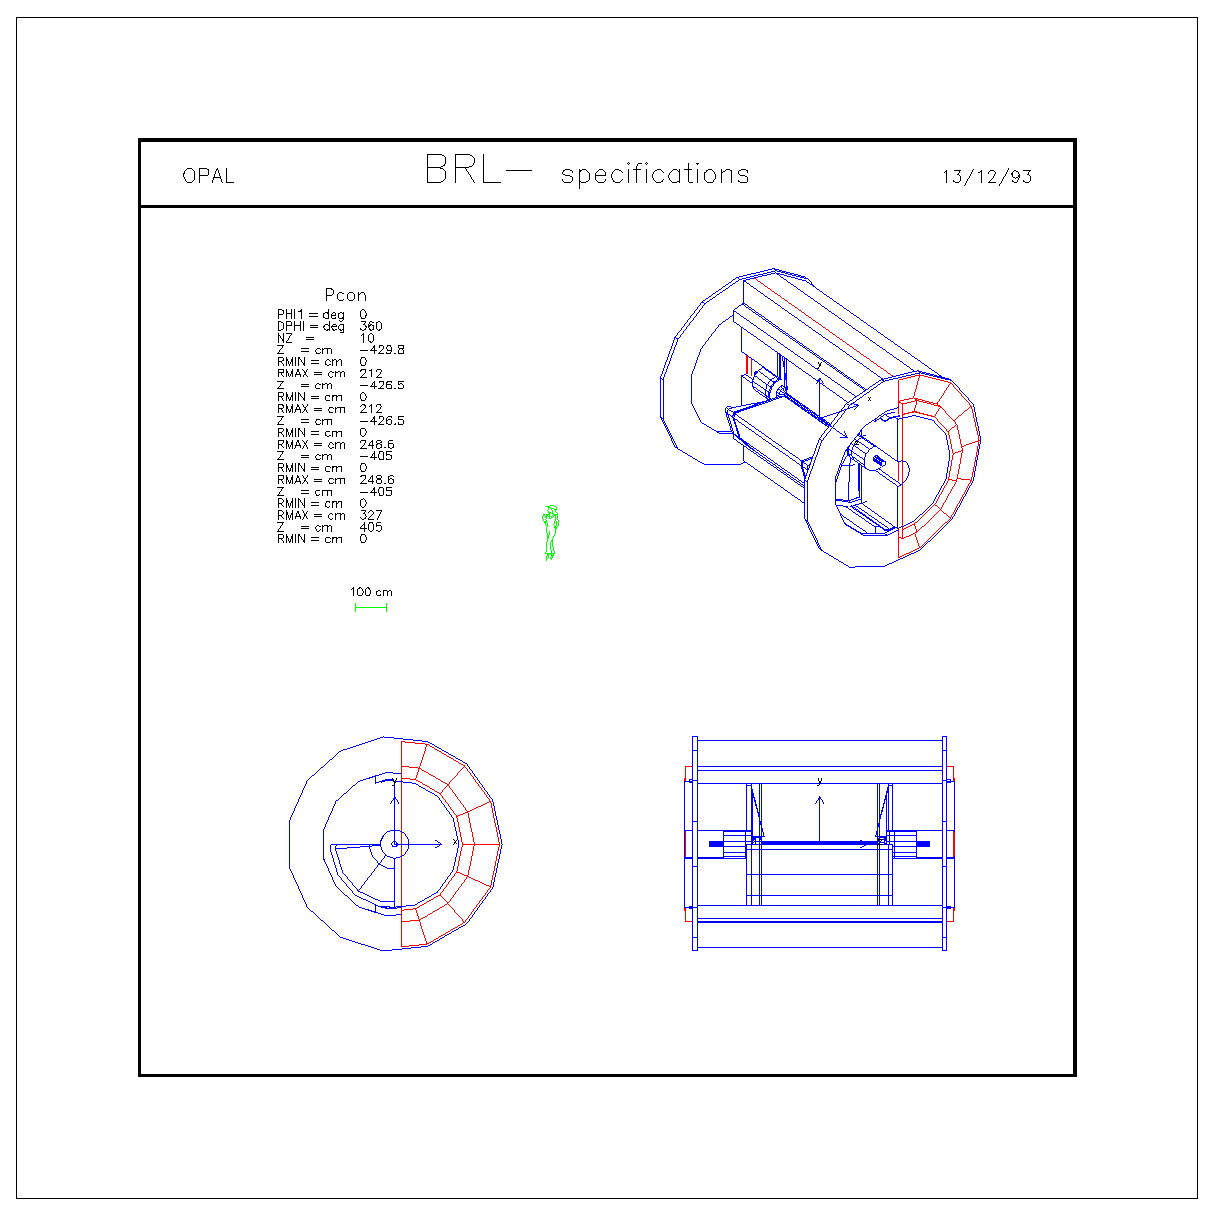
\epsfig{file=eps/draw220-2.eps,width=14cm}
     \caption{Example of use of {\tt GDSPEC}}
     \label{fg:draw220-2}
\end{figure}

\Shubr{GDFSPC}{(CHNAME,ISORT,INTER)}
Draws on separate pictures the full set of \Rind{GDSPEC} for the geometrical
tree starting from {\tt CHNAME}, i.e. calls \Rind{GDSPEC} for
the volume {\tt CHNAME} and for all its descendants.
\begin{DLtt}{MMMMMMMM}
\item[CHNAME] ({\tt CHARACTER*4}) volume name;
\item[ISORT] ({\tt INTEGER}) alphabetic sorting flag;
\begin{DLtt}{MMMM}
\item[$= 1$] all the volumes will be drawn in ascending alphabetic order
according to their name;
\item[$\neq 1$] the volumes will be drawn in the order in which they
have been created;
\end{DLtt}
\item[INTER] ({\tt INTEGER}) interactive/batch version flag;
\begin{DLtt}{MMMM}
\item[$= 1$] the routine will prompt the user at each plot
before doing a clear screen;
\item[$\neq 0$] the routine will clear automatically the screen 
before starting a new frame.
\end{DLtt}

{\bf Note:} {\tt INTER} should be set to 1 when using the interactive version 
of {\tt GEANT} and to any other value when using a batch version.
\end{DLtt}
